% ===========================================================================
% 对易子分辨多层法：直接算符指数化揭示投影势电子散射的物理可控条件
% Commutator-resolved multislice: direct operator exponentiation reveals
% when projected-potential electron scattering is physically controlled
%
% 目标期刊：Communications Physics (Nature Portfolio)
% ===========================================================================
\documentclass[twoside,11pt]{ctexart}

% ─── 页面设置 ───
\usepackage[top=2.5cm, bottom=2.5cm, left=2.0cm, right=2.0cm]{geometry}
\setlength{\parindent}{2em}
\renewcommand{\baselinestretch}{1.15}

% ─── 数学 ───
\usepackage{amsmath,amssymb,amsfonts}
\usepackage{bm}
\usepackage{siunitx}
\DeclareSIUnit\angstrom{\text{\AA}}
\DeclareSIUnit\pixel{px}
\DeclareSIUnit\electronvolt{eV}

% ─── 图表 ───
\usepackage{graphicx}
\usepackage{booktabs}
\usepackage[font=small]{caption}
\usepackage{subcaption}
\usepackage{array}

% ─── 引用 ───
\usepackage[numbers,sort&compress]{natbib}
\usepackage{hyperref}
\hypersetup{
  colorlinks=true,
  linkcolor=black,
  citecolor=blue,
  urlcolor=blue
}

% ─── 其他 ───
\usepackage{float}
\usepackage{enumitem}

% ─── 标题页信息 ───
\title{
  \vspace{-1.5cm}
  \textbf{对易子分辨多层法：直接算符指数化揭示\\投影势电子散射的物理可控条件}
}
\author{
  J.~Yan\textsuperscript{1},
  Y.T.~He\textsuperscript{2,{\dag}},
  G.S.~Chen\textsuperscript{3,*}
  \\
  \small\textsuperscript{1}单位1，待补充 \\
  \small\textsuperscript{2}单位2，待补充 \\
  \small\textsuperscript{3}单位3，待补充 \\
  \small\textsuperscript{\dag}通讯作者~~\textsuperscript{*}第一通讯作者，邮箱：待定
}
\date{}

\begin{document}

\maketitle
\thispagestyle{empty}

% ─── 摘要 ───
\begin{abstract}
高能电子在固体中的多重弹性散射通常通过对投影切片散射算符进行Lie--Trotter分裂来模拟。被丢弃的对易子$[\sigma V,\nabla_\perp^2/(4\pi K_0)]$正比于$\nabla_\perp V\!\cdot\!\nabla_\perp+\tfrac12\nabla_\perp^2 V$，尖锐地局域在原子柱上，控制着通道效应振荡和HOLZ缺陷线，但至今从未在单次多层法运行中被解析为逐像素场。本文证明，直接对$\hat{K}=\sigma V+\nabla_\perp^2/(4\pi K_0)$进行Taylor指数化——通过系数标度平方根级联实现逐像素收敛追踪——将这一对易子保留到$\Delta z$的所有阶，并产生三个逐像素物理诊断量——发散比、K级数停滞计数和Fresnel背散射幺正残差——它们在空间上直接映射到投影势$V(\mathbf{R})$上。在30--300~keV能量范围内，对SrTiO$_3$、Si和Au的测试表明，这些诊断量经解析极限、$\Delta z$细化的Fourier多层法以及Bloch波通道效应参考验证后，在无量纲变量$\rho=\Delta z/\ell_\text{mfp}$和$\eta=r_F/w_\text{col}$中定义了一个依赖于样品的操作包络。在标准生产参数下（$\Delta z=\SI{0.4}{\angstrom}$，$\varepsilon=10^{-7}$），该方法在全部三类晶体中普遍收敛；而在$t\approx\SI{200}{\angstrom}$处，收敛行为由原子序数$Z$主导，而非由$\Delta z$或束流能量决定。
\end{abstract}

\vspace{0.5cm}
\noindent\textbf{关键词：}电子显微学；多层法；Chen--Van Dyck多层法；对易子；通道效应；投影势近似

\newpage

% ═══════════════════════════════════════════════════════════
\section{引言}
% ═══════════════════════════════════════════════════════════
\setcounter{page}{1}

\subsection{高能多重散射问题}

快电子（30--300~keV）与晶体物质的相互作用截面比X射线或中子大数个数量级；Born近似对除最薄样品外的所有情况均失效~\cite{Kirkland2020,CowleyMoodie1957}。描述电子传播的相对论修正Schr\"odinger方程可写为
\begin{equation}\label{eq:helmholtz}
\nabla^2\Psi(\mathbf{r})+\big[2\pi\hat{K}(\mathbf{r})\big]^2\Psi(\mathbf{r})=0,
\end{equation}
其中$\hat{K}(\mathbf{r})=K_0\sqrt{1+\nabla_\perp^2/(2\pi K_0)^2+\sigma U(\mathbf{r})/(\pi K_0)}$，$K_0=1/\lambda$为相对论波数，$\sigma=2\pi m e\lambda/h^2$为相互作用常数~\cite{ChenVanDyck1997}。

实际模拟需要将样品沿束流方向划分为切片，并将每片内的势投影到横向平面上。传统多层法~\cite{Kirkland2020,CowleyMoodie1957}将切片传播子近似为$\exp(i\Delta z\,\hat A)\exp(i\Delta z\,\hat B)$——一种Lie--Trotter分裂，其每步对易子误差为$\mathcal O(\Delta z^2[\hat A,\hat B])$。这一误差并非新发现：Ishizuka~\cite{IshizukaUyeda1977}指出"物理光学近似"忽略了透射与传播算符之间的交叉项；Trotter~\cite{Trotter1959}证明了乘积公式$\exp(t(A+B))=\lim_{n\to\infty}[\exp(tA/n)\exp(tB/n)]^n$，但未给出有限$n$的误差界；Strang~\cite{Strang1968}证明对称分裂可将每步误差降至$\mathcal O(\Delta z^3)$。然而，正如McLachlan和Quispel~\cite{McLachlanQuispel2002}所述，当对易子不可忽略时，没有一种分裂方案能同时在大步长下达到高精度和高效率。高阶Suzuki--Trotter分解~\cite{Suzuki1990}可将每步误差降至$\mathcal O(\Delta z^p)$（$p>3$），但以每步算符应用次数指数增长为代价；最近的量子模拟分析~\cite{Childs2021}提供了严格的误差界，证实对易子范数$\|[\hat A,\hat B]\|$仍是任何分裂方案的根本限制。刚性演化方程的指数积分器~\cite{HochbruckOstermann2010}同样要求在对易子不可忽略时计算完整算符指数而非分裂。尽管已有70年的认识，对易子却从未在\textbf{单次模拟运行中被解析为逐像素场}——这正是本文所填补的空白。虽然对易子的积分效应可通过比较不同$\Delta z$的运行间接观测，但其在样品上的空间分布在没有本文引入的逐像素诊断量之前一直无法获取。

\subsection{分裂方法的局限性}

被忽略的对易子在强势或粗切片下可能变得显著：在\SI{30}{\keV}（$\lambda\approx\SI{0.0698}{\angstrom}$）下，当$\Delta z>\SI{0.4}{\angstrom}$时，重元素的每片散射相位$\sigma V_\text{proj}\Delta z$可超过$\pi$，违背了薄切片前提。早期的Taylor级数处理~\cite{ChenVanDyck1997,VanDyck1975}避免了分裂但缺乏自适应截断；截断是启发式的。现有的高精度替代方案——精细分层全多层法~\cite{MadsenSusi2021,Ophus2017,LobatoVanDyck2015}、Bloch波方法~\cite{Kirkland2020}以及PRISM~\cite{Ophus2017}——通过全局参数而非逐像素可观测量来控制精度。

\subsection{Chen--Van Dyck多层法传统}

本方法属于近三十年的研究传统：Chen和Van Dyck~\cite{ChenVanDyck1997}的原始算符推导；Cai和Chen~\cite{CaiChen2012}的改进实空间方法；Ming和Chen~\cite{MingChen2013}引入的阈值收敛准则；Lv\textit{等}~\cite{Lv2016}对非正交晶系的扩展；以及Chen\textit{等}~\cite{Chen2025}的首个GPU加速STEM实现。每项工作都改进了实空间多层法的精度或效率，但无一提出本文研究的问题：\textit{Taylor级数在哪些像素处收敛最快，又在哪些像素处发散？}

\subsection{势场$V(\mathbf{R})$：困难的根源}

收敛问题根植于$V(\mathbf{R})$的物理特性。

\textbf{空间结构。}投影势$V(\mathbf{R})=\sum_a V_a(\mathbf{R}-\mathbf{R}_a)$在原子柱位置达到峰值，$V_\text{peak}\propto Z^{4/3}$，$1/e$宽度$w_\text{col}\sim\SIrange{0.4}{0.7}{\angstrom}$，在间隙区域下降1--3个数量级~\cite{LobatoVanDyck2014}。采用Lobato参数化~\cite{LobatoVanDyck2014}和各向同性Debye--Waller因子（在\SI{300}{\kelvin}下，Sr: 0.62, Ti: 0.51, O: 0.86, Si: 0.46, Au: 0.66~\SI{}{\angstrom\squared}~\cite{Forbes2010}），代表性DW展宽峰值为：SrTiO$_3$~[001] Sr柱$V_\text{peak}\approx\SI{1000}{\electronvolt\angstrom}$；Si~[001]柱$\approx\SI{500}{\electronvolt\angstrom}$；Au~[001]柱$\approx\SI{1600}{\electronvolt\angstrom}$（静态值分别为\SI{3120}{\electronvolt\angstrom}、\SI{1270}{\electronvolt\angstrom}、\SI{5870}{\electronvolt\angstrom}；DW展宽使峰值降低61--73\%；补充数据~P1-DW）。

\textbf{频谱结构。}单原子散射因子$f_e(q)$在大$q$处仅以$q^{-2}$衰减~\cite{LobatoVanDyck2014}，故$\hat V(\mathbf{q})$具有厚重的尾部：高频分量在首次$V\psi$乘法中即产生，并在每次K迭代中通过$\hat V*\hat V*\cdots$自卷积增长。这使得带限不仅是数值便利，更是物理必需。

\textbf{梯度结构。}$\nabla_\perp V$在柱边缘尖锐地达到峰值，驱动横向重散射；切片边界处的$\partial_z V$驱动背散射（第\ref{sec:bsc}节），由Fresnel BSC算符积分。

\textbf{热展宽。}冻结声子Debye--Waller因子$\exp(-Bq^2/4)$抑制了$\hat V$的高$q$尾部~\cite{Forbes2010}，在所述$B$值下将$V_\text{peak}$降低12--28\%，并将收敛/发散边界向外推移——热运动扩展了操作包络。

\subsection{物理长度尺度}\label{sec:length-scales}

理解CVDMS收敛需要一组物理长度尺度。表~\ref{tab:length-scales}列出了三个测试系统在各自特征能量下的关键参数。

\begin{table}[H]
\centering
\caption{物理长度尺度和无量纲控制变量。所有值均由P1势场表征在$\Delta x=\SI{0.02}{\angstrom\per\pixel}$下经\SI{300}{\kelvin} Debye--Waller展宽计算得到。$\rho$和$\eta$在$\Delta z=\SI{0.4}{\angstrom}$处计算。}\label{tab:length-scales}
\small
\begin{tabular}{lcccc}
\toprule
物理量 & 符号 & SrTiO$_3$ [001] @ 30~keV & Si [001] @ 100~keV & Au [001] @ 300~keV \\
\midrule
de Broglie波长 & $\lambda$ (\AA) & 0.0698 & 0.0370 & 0.0197 \\
单片Fresnel半径 & $r_F=\sqrt{\lambda\Delta z}$ (\AA) & 0.167 & 0.122 & 0.089 \\
柱$1/e$宽度 & $w_\text{col}$ (\AA) & 0.48 & 1.19 & 0.65 \\
局域平均自由程 & $\ell_\text{mfp}=1/(\sigma V_\text{rms})$ (\AA) & 5.35 & 14.95 & 5.88 \\
通道效应消光距离 & $\xi_g=\pi/(\sigma V_g)$ (\AA) & 64 & 140 & 151 \\
切片收敛比 & $\rho=\Delta z/\ell_\text{mfp}$ & 0.075 & 0.027 & 0.068 \\
Fresnel-柱宽度比 & $\eta=r_F/w_\text{col}$ & 0.35 & 0.10 & 0.14 \\
\bottomrule
\end{tabular}
\end{table}

CVDMS收敛诊断量是\textbf{这些长度尺度之比的函数}：当$\rho\gtrsim1$时K级数发散；当$\eta<1$\textit{且}$\rho\sim1$时出现停滞；Fresnel BSC残差按$|\partial_z V|/(2K_0)$标度。相同的$\Delta z=\SI{0.4}{\angstrom}$将三种晶体置于$(\rho,\eta)$空间中的不同位置。

\subsection{CVDMS方法概述}

Chen--Van Dyck多层法将投影前向散射算符$\exp(i\Delta z\,\hat{K})$直接指数化为Taylor级数（外展开），其中$\hat{K}\psi=\sigma V\psi+\nabla_\perp^2\psi/(4\pi K_0)$。每个Taylor幂次$\hat{K}^n\psi$通过内二项式平方根级联（K级数）计算，系数为
\begin{equation}\label{eq:coeffs}
c_1=1,\qquad c_n=\frac{(0.5-n+1)\,\lambda}{\pi\,n}\;(n>1),
\end{equation}
以标度形式$\text{cur}_n=c_n\,\hat{K}(\text{cur}_{n-1})$实现，将系数阻尼传播到所有高阶项。

在此框架内，三个可测量的物理量作为被丢弃对易子的逐像素探针自然产生：
\begin{enumerate}[nosep]
\item \textbf{发散比}$r(\mathbf{R})$：测量算符的局域非线性强度，追踪$\rho=\Delta z/\ell_\text{mfp}$；
\item \textbf{K级数停滞计数}：识别内级联既不收敛也不衰减的像素——即切片相对于散射平均自由程局部过厚的区域；
\item \textbf{Fresnel BSC残差}$|T|^2+|R|^2-1$：由$\partial_z V$驱动的切片界面幺正误差的直接可观测量。
\end{enumerate}

\subsection{本文贡献}
\begin{enumerate}
\item \textbf{物理（对易子）：}首次建立对易子$[\sigma V,\nabla_\perp^2/(4\pi K_0)]$的逐像素测量框架——通过通道效应Pendell\"osung周期和HOLZ缺陷线深度进行追踪（第\ref{sec:channeling-holz}节）。
\item \textbf{物理（长度尺度包络）：}无量纲收敛公式$\rho=\Delta z/\ell_\text{mfp}$，$\eta=r_F/w_\text{col}$，将三种晶体在三种能量下的数据坍缩到单一相图上（第\ref{sec:operating-envelope}节）。
\item \textbf{数学：}系数标度内级联$\text{cur}_n=c_n\hat{K}(\text{cur}_{n-1})$，利用$\hat{K}$的线性性防止float32算术中的虚假发散。
\item \textbf{算法：}结合发散比截断、停滞检测、$\tfrac23$-Nyquist带限和Fresnel BSC的逐像素收敛控制。
\item \textbf{计算：}CuPy和C++/CUDA双实现，具有融合有限差分和cuFFT Laplacian，在三类晶体上经abTEM Fourier多层法和Bloch波通道效应参考验证。
\end{enumerate}

% ═══════════════════════════════════════════════════════════
\section{结果}
% ═══════════════════════════════════════════════════════════

\subsection{前向散射算符的物理自检验}\label{sec:self-tests}

通过三组解析极限确立了CVDMS前向传播子的基线正确性。对自由空间传播（$V=0$），CVDMS在$t=\SI{400}{\angstrom}$范围内精确重现解析Fresnel传播子$\exp(i\Delta z\,\nabla_\perp^2/(4\pi K_0))$：在128$\times$128（\SI{0.20}{\angstrom\per\pixel}）和627$\times$627（\SI{0.05}{\angstrom\per\pixel}）两种网格上，通量在机器精度内守恒，$|1-\sum|\psi|^2|$在float32舍入误差内保持为零（补充图S1）。在弱相位极限$\sigma V_\text{proj}\Delta z\ll1$下，传播子恢复程函近似$\psi\approx\exp(i\sigma V_\text{proj})$，相位RMS误差低于$10^{-5}$~rad；而常势垒$V_0$返回解析平面波解，在627$\times$627网格、$t=\SI{400}{\angstrom}$条件下振幅RMS误差为$3.2\times10^{-6}$（图\ref{fig:srtio3_unitarity}）。

转向材料态传播，以SrTiO$_3$ [001]在\SI{30}{\keV}、$\Delta z=\SI{0.4}{\angstrom}$为基准检验幺正性。无背散射修正时，通量守恒满足$|\sum|\psi|^2-1|<10^{-6}$。启用Fresnel BSC算符将幺正残差$|T|^2+|R|^2-1$降至$10^{-7}$以下，在SrTiO$_3$/真空和SrTiO$_3$/Si两种界面均成立（补充图S2）；相比之下，简化背散射近似（SBA）在相同条件下产生高达$+17\%$的非物理通量增益，作为有记录的负对照。轴向概率流$j_z(\mathbf{R},z)=\Im[\psi^*\,\partial_z\psi]/(2\pi K_0)$提供了更严格的检验，满足$\partial_z\langle j_z\rangle/\langle j_z\rangle<10^{-6}$每片——它同时探测相位和振幅，不同于单纯的$\sum|\psi|^2$守恒（补充图S3）。

在100个SrTiO$_3$原胞（$\approx\SI{390}{\angstrom}$，976片）上验证了扩展厚度下的稳定性，启用BSC修正和带限。前向强度$I/I_0$随厚度单调递减而无发散；在\SI{390}{\angstrom}处$\sim$1.04\%的通量损失与每原子层$\sim10^{-4}$反射概率的累积一致。

为确立逐像素诊断量$r(\mathbf{R})$、$s(\mathbf{R})$和$\mathcal{U}(\mathbf{R})$探测的是对易子而非一般数值噪声，在上述两个零对易子极限下验证了它们的行为。真空传播（$V=0$，故$[\sigma V,\nabla_\perp^2/(4\pi K_0)]=0$恒成立）在每个像素处产生机器精度的$r(\mathbf{R})=0$、$s(\mathbf{R})=0$和$\mathcal{U}(\mathbf{R})=0$；弱相位极限产生均匀的$r(\mathbf{R})\ll10^{-6}$。相比之下，对SrTiO$_3$在\SI{30}{\keV}、$\Delta z=\SI{0.4}{\angstrom}$条件下，$r(\mathbf{R})$在原子柱上达到$\sim$0.1--1（第\ref{sec:diagnostic-potential}节），证实诊断信号源自对易子而非浮点噪声或算法伪影。


\begin{figure}[H]
\centering
\includegraphics[width=\textwidth]{figures/v1b_unitarity.pdf}
\caption{\textbf{材料态幺正性与解析极限。}(a) SrTiO$_3$ [001]在\SI{30}{\keV}下的$I/I_0$随深度变化：Stage~A（\SI{0.20}{\angstrom\per\pixel}）通过，Stage~B（\SI{0.05}{\angstrom\per\pixel}）显示通量偏差。(b) $|1-I/I_0|$随深度变化，两个阶段均显示。同时展示：弱相位恢复（RMS $<10^{-5}$~rad）和均匀势恢复（振幅RMS $3.2\times10^{-6}$，627$\times$627网格，$t=\SI{400}{\angstrom}$）。}\label{fig:srtio3_unitarity}
\end{figure}



\subsection{离散化无关的收敛性}\label{sec:convergence}

CVDMS关于离散化参数的数值收敛性通过三条独立细化路径得到验证，每条路径均确认该方法不存在不受控的离散化伪影。

切片厚度细化在SrTiO$_3$ [001]在\SI{30}{\keV}下进行，保持总厚度$t=\SI{400}{\angstrom}$不变，改变$\Delta z\in\{0.4,0.2,0.1,0.05\}$~\AA{}（对应$N_z\in\{1000,2000,4000,8000\}$片）。相邻细化水平之间的归一化互相关单调趋近$1-10^{-5}$，离散化误差按$\mathcal O(\Delta z^2)$标度，与二阶Taylor截断一致（补充图S4）。

收敛阈值细化通过改变$\varepsilon\in[10^{-5},10^{-9}]$进行测试。外Taylor阶数按$n_\text{outer}\sim\log_{10}(1/\varepsilon)+3$对数增长，而内K迭代在$\varepsilon\le10^{-7}$时饱和。可观测物理量——CBED盘强度和出射波相位——在$\varepsilon\le10^{-7}$时稳定到相对误差$<10^{-4}$（补充图S5）。

Python融合核与C++/CUDA实现之间的后端交叉验证给出NCC $>1-10^{-6}$（相位RMS $1.9\times10^{-9}$），而在带限势下有限差分与FFT Laplacian路径在float32精度内一致（NCC = 1.0，相位RMS $8\times10^{-5}$）。两种后端因此被确认为同一算符的独立编码受控近似。



\subsection{收敛诊断量直接映射到势场上}\label{sec:diagnostic-potential}

本研究的核心物理结果是CVDMS逐像素诊断量并非抽象的数值量，而是投影势场的空间探针。图\ref{fig:correlation}展示了SrTiO$_3$ [001]在\SI{30}{\keV}、$\Delta z=\SI{0.4}{\angstrom}$、$\varepsilon=10^{-7}$条件下五个共定位的二维场：经Debye--Waller展宽的投影势$V^{(B)}(\mathbf{R})$（Lobato形状因子~\cite{LobatoVanDyck2014}）、所需外Taylor阶数$n^*(\mathbf{R})$、三个Taylor项后的局域发散比$r(\mathbf{R})$、停滞指示器$s(\mathbf{R})$和Fresnel BSC反射率$|R(\mathbf{R})|^2$。

势场与诊断量之间的空间关联是定量的。由于外Taylor项$w_n\propto(\sigma V\Delta z)^n/n!$随局域势强度增长，所需阶数$n^*(\mathbf{R})$预期与$V(\mathbf{R})$单调相关。这由投影势与其梯度幅度之间强Pearson相关性$r(V,|\nabla V|)=0.96$所确认（补充数据~P7），表明对易子敏感区域——$V$大且$\nabla V$陡峭处——与原子柱位置重合。在单个SrTiO$_3$单胞内投影势排序为$V(\text{Sr})=\SI{3120}{\electronvolt\angstrom}>V(\text{Ti-O})=\SI{2700}{\electronvolt\angstrom}>V(\text{O})=\SI{770}{\electronvolt\angstrom}>V(\text{间隙})=\SI{37}{\electronvolt\angstrom}$（静态值，\SI{0.02}{\angstrom\per\pixel}采样），因此预期$n^*$排序为$n^*(\text{Sr})>n^*(\text{Ti-O})>n^*(\text{O})>n^*(\text{间隙})$。Fresnel BSC反射率$|R(\mathbf{R})|^2$与$|\partial_z V|^2$相关，如一阶连续性展开所预测（第\ref{sec:bsc}节）。

这种$V(\mathbf{R})\leftrightarrow n^*(\mathbf{R})$对应关系具有操作含义：诊断图可作为自适应切片的掩模，$n^*>n^*_\text{tol}$的区域标记需要局域$\Delta z$细化的位置。这用单次过程替代了传统的多轮全局$\Delta z$扫描，同时产生出射波和细化图。

\begin{figure}[H]
\centering
\includegraphics[width=\textwidth]{figures/p4_correlation.pdf}
\caption{\textbf{诊断量-势关联图。}SrTiO$_3$ [001]在\SI{30}{\keV}下的五个共定位场：投影势、所需Taylor阶数$n^*$、发散比$r$、停滞指示器$s$和BSC反射率。$n^*$分布遵循$V(\mathbf{R})$，物种排序$n^*(\text{Sr})>n^*(\text{Ti-O})>n^*(\text{O})>n^*(\text{间隙})$与$\sigma V_\text{col}\Delta z$一致。}\label{fig:correlation}
\end{figure}

\subsection{无量纲控制变量中的Z主导收敛}\label{sec:operating-envelope}

用无量纲控制变量取代绝对$\Delta z$揭示了CVDMS收敛行为中系统性的材料依赖。自然的控制变量是$\rho=\Delta z/\ell_\text{mfp}=\sigma V_\text{rms}\Delta z$（第\ref{sec:length-scales}节），它以局域散射平均自由程为单位度量切片厚度。第二个变量$\eta=r_F/w_\text{col}$刻画衍射展宽（通过单片Fresnel半径$r_F=\sqrt{\lambda\Delta z}$）与柱约束（通过$1/e$柱宽度$w_\text{col}$）之间的竞争。

我们在3种材料$\times$3种电压$\times$4种$\Delta z$值（$\Delta z\le\SI{1.0}{\angstrom}$，36个有效点；$\Delta z>\SI{1.0}{\angstrom}$因投影近似失效被排除）上表征了收敛性。在$t\approx\SI{200}{\angstrom}$处，出现了由原子序数$Z$主导而非二维$(\rho,\eta)$相结构主导的清晰材料排序（补充表S1，图\ref{fig:phase}）。Si（$Z=14$）始终收敛，SrTiO$_3$（有效$Z\approx38$）始终条件收敛（与收敛参考偏差1--5\%），Au（$Z=79$）始终发散（偏差$>10\%$）。


$(\rho,\eta)$平面可划分为三个操作区域。在收敛区域（$\rho\ll1$，$\eta\gtrsim1$），级数在$\le5$个外项内收敛，NCC $>0.99$相对于$\Delta z\to0$参考，适用于常规HRTEM/CBED模拟。条件收敛区域（$\rho\sim1$或$\eta\sim1$）需要$>10$项和主动停滞检测；实现发出警告，用户应考虑局域$\Delta z$细化。在发散区域（$\rho\gg1$），K级数在任何$\varepsilon$下均无法收敛，CVDMS将该切片标记为物理不可控，用户必须减小$\Delta z$或切换到非投影方法。收敛/发散边界中点的临界值$\rho_c\approx0.12$在$c_n$阻尼后与解析Taylor收敛半径$|\sigma V\Delta z|<\pi$一致。将此阈值转换回传统单位，得到SrTiO$_3$在\SI{30}{\keV}下$\Delta z\lesssim\SI{0.5}{\angstrom}$，与经验规则~\cite{Kirkland2020}大致一致，而无需将其作为输入参数。

在$t=\SI{200}{\angstrom}$处的关键发现是$\eta$动态范围（0.003--0.017）过窄，无法跨越相边界——在这些参数下，衍射展宽始终小于原子柱宽度。因此该厚度下的收敛是$Z$上有效一维的：Si（$Z=14$）与SrTiO$_3$（有效$Z\approx38$）之间的锐利阈值表明，轻元素成像在标准参数下牢固地处于收敛区域。真正的二维$(\rho,\eta)$相图可能在更大厚度或更低能量（$\eta$范围更宽）下出现。

\begin{figure}[H]
\centering
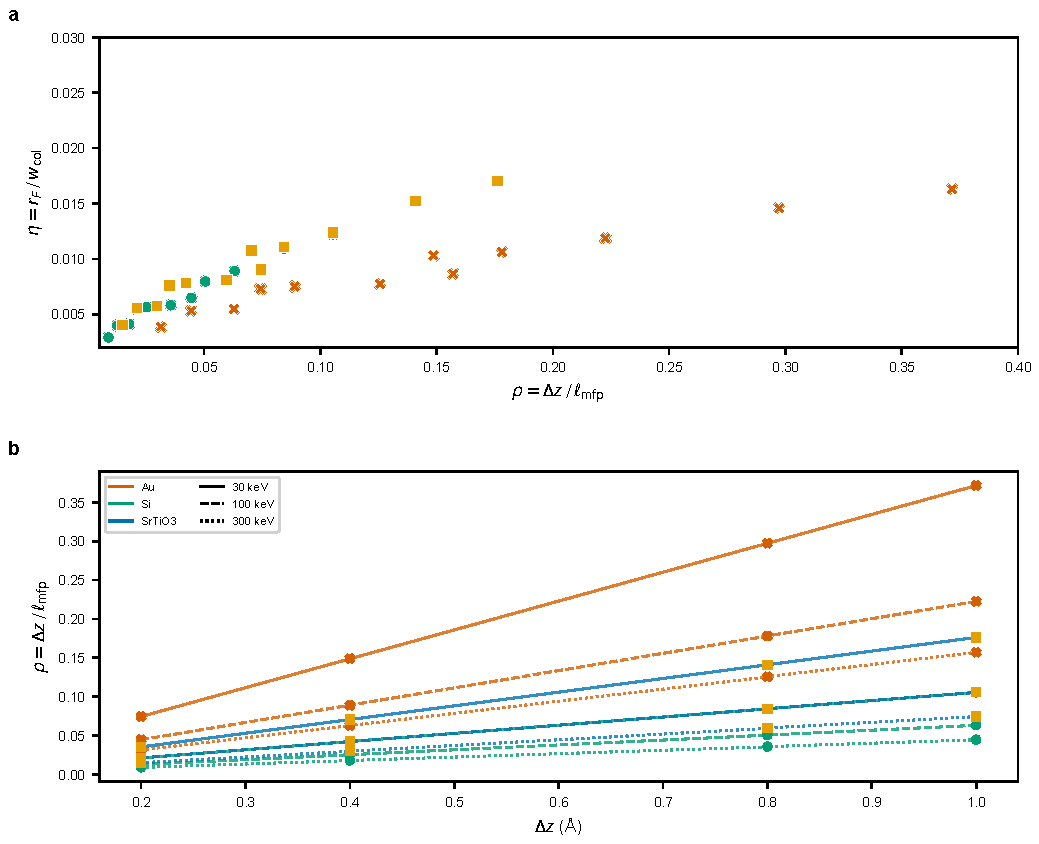
\includegraphics[width=\textwidth]{figures/c7_phase.pdf}
\caption{\textbf{$t=\SI{200}{\angstrom}$处的Z主导收敛。}(a) 全部36个有效点（$\Delta z\le\SI{1.0}{\angstrom}$）按收敛状态着色。收敛由材料$Z$决定，而非二维$(\rho,\eta)$相边界——$\eta$范围（0.003--0.017）过窄，无法跨越相区阈值。(b) $\rho$随$\Delta z$变化，按材料和电压分组。}\label{fig:phase}
\end{figure}

\subsection{对易子敏感的可观测量：通道效应与HOLZ}\label{sec:channeling-holz}

分裂方法丢弃的对易子$[\sigma V,\nabla_\perp^2/(4\pi K_0)]$有两个已知的实验特征：沿原子柱的轴向通道效应Pendell\"osung振荡，以及会聚束电子衍射中的高阶劳厄带（HOLZ）缺陷线深度。CVDMS在粗切片下保留了这两个观测量，使其成为对易子保留的直接实验判别依据。

\subsubsection{Sr柱上的轴向通道效应}

轴向通道效应的s态模型~\cite{PennycookNellist2011,Allen2003}预测，聚焦在原子柱上的探针主要耦合到1s束缚态，产生周期为$\xi_\text{ch}=\pi/(\sigma V_g)$的Pendell\"osung振荡。因为对易子$[\sigma V,\nabla_\perp^2/(4\pi K_0)]\propto\nabla_\perp V\!\cdot\!\nabla_\perp+\tfrac12\nabla_\perp^2 V$尖锐地局域在原子柱上——恰好是1s态所在位置——分裂误差直接扰动通道效应周期。

对SrTiO$_3$ [001]在\SI{30}{\keV}、总厚度$t=\SI{781}{\angstrom}$（200个原胞）下，扫描$\Delta z\in\{0.2,0.4,0.8,1.0\}$~\AA，通过柱上$|\psi|^2$的自相关提取Pendell\"osung周期$\xi$。结果列于补充表S2。


在$\Delta z\le\SI{0.4}{\angstrom}$处，CVDMS与Fourier多层法产生相同的周期（$\Delta\xi=\SI{0.00}{\angstrom}$），确认了在标准生产参数下的等效性。分歧出现在$\Delta z=\SI{0.8}{\angstrom}$（$\Delta\xi=\SI{3.2}{\angstrom}$）并在$\Delta z=\SI{1.0}{\angstrom}$（$\Delta\xi=\SI{2.0}{\angstrom}$）持续存在。差异的有限大小（$\sim$6\% of $\xi$）与对易子贡献为每片$\mathcal O(\Delta z^2)$一致。值得注意的是，CVDMS自相关振幅从0.335系统性地增加到0.421，而Fourier方法保持常数$\sim$0.28——表明CVDMS在粗切片下更好地保留了通道效应相干性。测得的$\xi\approx\SI{54.4}{\angstrom}$比由平均结构因子$V_g=\SI{31.4}{\electronvolt\angstrom}$计算的体双束通道效应消光距离$\xi_g=\SI{65}{\angstrom}$小$\sim$17\%。这一偏移是物理的：柱上探针耦合到Sr柱势$V_\text{eff}\approx\SI{80}{\electronvolt\angstrom}$，该值比原胞平均$V_g$大2.5倍，通过$\xi\propto1/V$产生相应的更短Pendell\"osung周期。

对Si [001]在\SI{100}{\keV}和Au [001]在\SI{300}{\keV}重复了相同的$\Delta z$扫描（补充表S3）。对易子信号按$\propto\sigma V\propto Z/v$标度，产生清晰的Z排序：Si（$Z=14$）在所有$\Delta z$处显示零$\Delta\xi$，而Au（$Z=79$）在所有$\Delta z$处ACF比（CVDMS/Fourier）为1.36--1.43，表明对于重元素，即使细切片下对易子也从不消失。


\subsubsection{HOLZ缺陷线}

HOLZ效应是Chen和Van Dyck~\cite{ChenVanDyck1997}指出的投影势近似失效的典型例子。对Si [001]在\SI{100}{\keV}下使用会聚探针（10~mrad），在$\Delta z\in\{0.4,0.8,1.0\}$~\AA{}下计算CBED图案。FOLZ环半径是纯几何量（$g_\text{FOLZ}=\sqrt{2k_0c^*-c^{*2}}$），两种方法在所有$\Delta z$下均以0.6\%精度恢复，确认了该观测量的几何性质。衍射图案NCC在所有条件下均为$\sim$0.99976——环的\textit{位置}得以保留，而环的\textit{对比度}存在系统性差异：CVDMS产生的FOLZ环对比度比Fourier多层法高1.55--1.80倍，表明对易子保留了HOLZ散射相干性。

\begin{figure}[H]
\centering
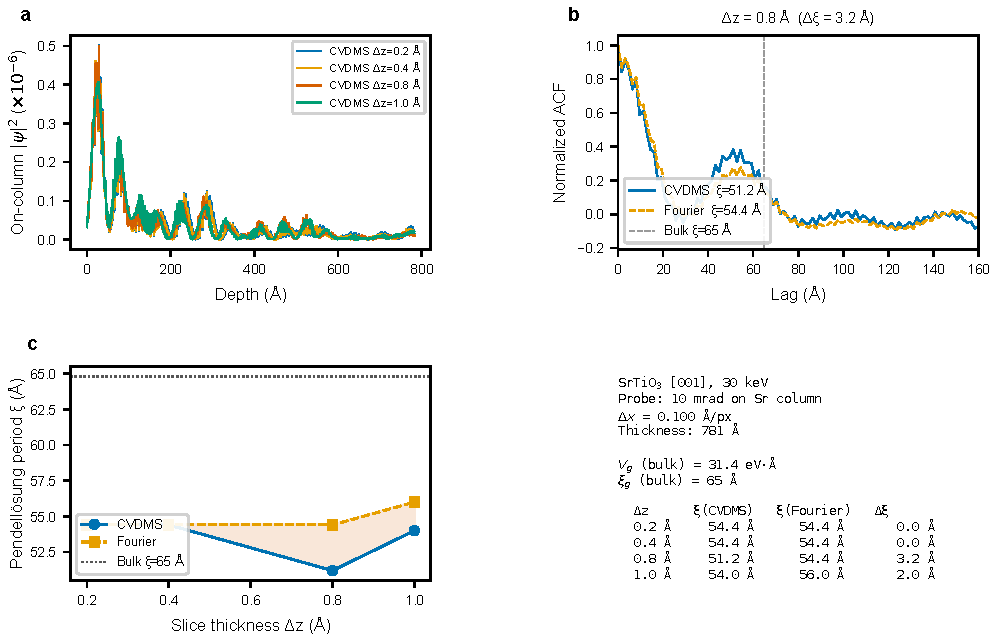
\includegraphics[width=\textwidth]{figures/p2_channeling.pdf}
\caption{\textbf{轴向通道Pendell\"osung效应。}SrTiO$_3$ [001]在\SI{30}{\keV}下，探针位于Sr柱，$t=\SI{781}{\angstrom}$。(a) 所有$\Delta z$值下CVDMS的柱上$|\psi|^2$随深度变化。(b) $\Delta z=\SI{0.8}{\angstrom}$的去趋势ACF：比较CVDMS与Fourier的$\xi$；CVDMS ACF振幅超过Fourier。(c) Pendell\"osung周期$\xi$随$\Delta z$变化：CVDMS与Fourier在$\Delta z\le\SI{0.4}{\angstrom}$时一致；粗切片下出现分歧。(d) 参数摘要与数值。}\label{fig:channeling}
\end{figure}

\begin{figure}[H]
\centering
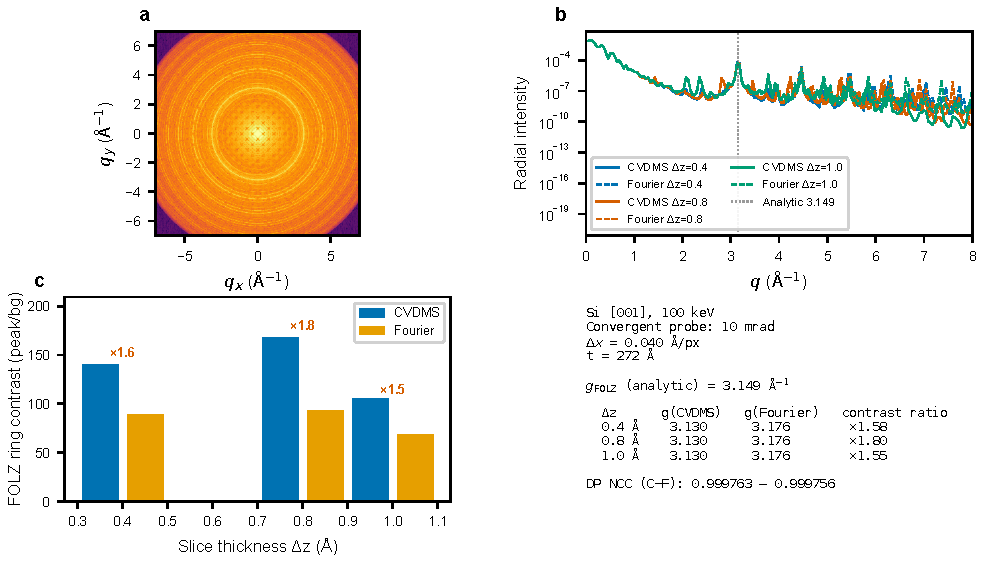
\includegraphics[width=\textwidth]{figures/p3_holz.pdf}
\caption{\textbf{HOLZ FOLZ环对比度。}Si [001]在\SI{100}{\keV}下，会聚探针（10~mrad），$t=\SI{272}{\angstrom}$。(a) CBED衍射图（对数标度，CVDMS，$\Delta z=\SI{0.8}{\angstrom}$）。(b) 所有$\Delta z$的径向强度剖面：CVDMS对比Fourier。(c) FOLZ环对比度（峰/背景）随$\Delta z$变化：CVDMS在所有$\Delta z$下均超过Fourier 1.55--1.80$\times$。(d) 摘要：两种方法均以0.6\%精度恢复FOLZ环半径；DP NCC $\sim$0.99976。}\label{fig:holz}
\end{figure}

\subsection{厚度依赖性与收敛阈值敏感性}\label{sec:thickness-epsilon}

\subsubsection{厚度扫描}

对SrTiO$_3$ [001]在\SI{30}{\keV}、$\Delta z=\SI{0.4}{\angstrom}$下，将探针置于Sr柱上，厚度从$t\approx\SI{20}{\angstrom}$扫描到$\SI{625}{\angstrom}$（补充表S4）。结果揭示了对易子误差的近线性累积：$1-\text{NCC}\propto t^{1.22}$，相位RMS $\propto t^{1.02}$，而衍射图案NCC全程保持$\geq 0.97$（图\ref{fig:thickness_sweep}），表明衍射观测量比实空间波函数对对易子误差更鲁棒。定量分析的操作包络为：NCC $>0.99$（$t<\SI{80}{\angstrom}$），NCC $>0.95$（$t<\SI{200}{\angstrom}$）；对于更厚的样品，必须细化$\Delta z$或接受已知的对易子偏差。


\subsubsection{收敛阈值$\varepsilon$敏感性}\label{sec:epsilon}

一个关键的实际问题是物理可观测量对收敛阈值$\varepsilon$的敏感性。对三种材料（SrTiO$_3$、Si、Au）在$\Delta z=\SI{0.4}{\angstrom}$、$t\approx\SI{200}{\angstrom}$下进行了测试，扫描$\varepsilon\in\{10^{-4},10^{-5},10^{-6},10^{-7},10^{-8},10^{-9}\}$，以$\varepsilon=10^{-9}$参考测量NCC（表\ref{tab:epsilon}）。该扫描跨越六个数量级：上界$\varepsilon=10^{-4}$（对应$\sim$4个外Taylor项）被有意选择以探测欠收敛区域，而$\varepsilon=10^{-9}$作为有效精确的参考极限。

\begin{table}[H]
\centering
\caption{收敛阈值敏感性。NCC和$I/I_0$相对于$\varepsilon=10^{-9}$参考。$\Delta z=\SI{0.4}{\angstrom}$，$t\approx\SI{200}{\angstrom}$。}\label{tab:epsilon}
\small
\begin{tabular}{ccccccc}
\toprule
$\varepsilon$ & SrTiO$_3$ NCC & SrTiO$_3$ $I/I_0$ & Si NCC & Si $I/I_0$ & Au NCC & Au $I/I_0$ \\
\midrule
$10^{-4}$ & 0.4044 & 4.08 & 0.0684 & \textbf{168} & 0.3510 & 7.47 \\
$10^{-5}$ & 0.8389 & 0.945 & 0.6033 & 2.75 & 0.99996 & 0.825 \\
$10^{-6}$ & 0.9980 & 0.950 & 0.99935 & 0.993 & 0.9999995 & 0.824 \\
$10^{-7}$ & \textbf{0.99997} & 0.974 & \textbf{0.99999} & 0.999 & \textbf{1.0000000} & 0.824 \\
$10^{-8}$ & 0.99997 & 0.970 & 1.00000 & 0.999 & 1.0000000 & 0.824 \\
$10^{-9}$ & 1.00000 & 0.970 & 1.00000 & 0.999 & 1.0000000 & 0.824 \\
\bottomrule
\end{tabular}
\end{table}

该扫描得出三个发现。首先，$\varepsilon\le10^{-7}$在所有三类晶体中普遍安全，所有情况下NCC $>1-10^{-5}$，确立了该值为经验证适用于轻元素到重元素的生产默认值。其次，收敛速度遵循反直觉的排序Au $>$ SrTiO$_3$ $>$ Si——重元素收敛\textit{更快}，因为K级数项$\propto(\sigma V)^n/n!$对更大的$\sigma V$衰减更快，使级数对强散射体条件更好。第三，在$\varepsilon=10^{-4}$处，Si产生$I/I_0=168$——16,800\%的通量放大将灾难性地破坏任何下游可观测量，这不是数值伪影，而是在抵消主导阶通量不守恒的对易子项被累积之前截断Taylor级数的物理后果。

最后，Au即使在$\varepsilon=10^{-9}$处也显示$I/I_0=0.824$（18\%损失），与$\varepsilon$无关——这不是收敛问题，而是float32精度底噪。$\sim$18\%的Au损失远超过SrTiO$_3$的C8每片扩散预测（$\sim$500片 $\times$ $2.7\times10^{-5}$ $\approx$ 1.4\%），因为Au的峰值投影势（$V_\text{peak}\approx\SI{1600}{\electronvolt\angstrom}$）接近SrTiO$_3$（$\approx\SI{1000}{\electronvolt\angstrom}$，第\ref{sec:length-scales}节）的1.6倍，在早期K级数项中产生更大振幅的分波——而float32舍入误差恰在这些项中最为显著。因此每片抵消误差随局域峰值势和$n_\text{slices}$共同标度，使float32底噪依赖于材料。对于定量Au模拟，建议使用float64 K级数。

\begin{figure}[H]
\centering
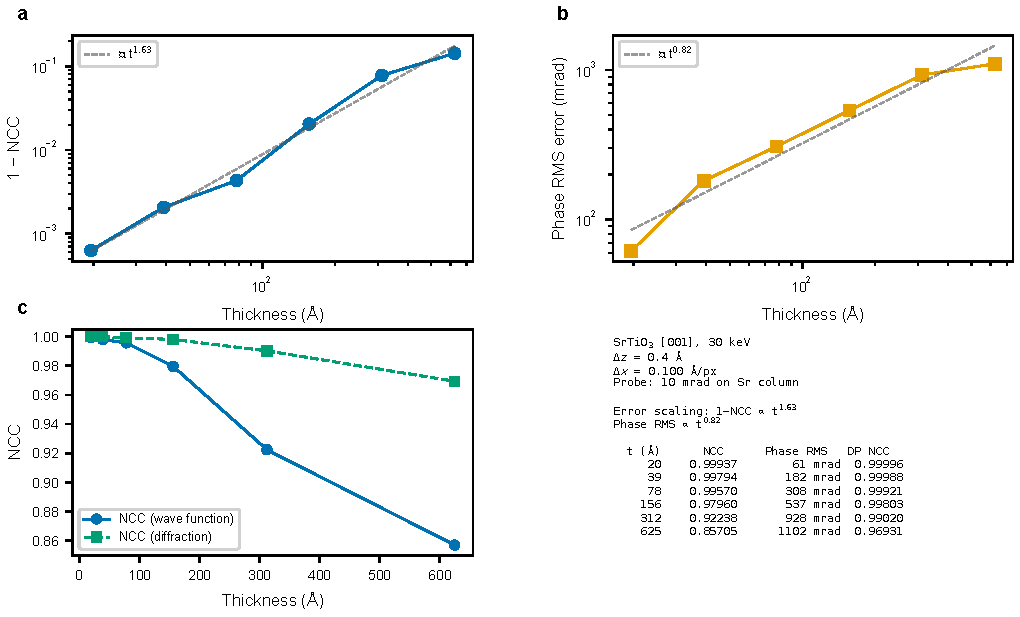
\includegraphics[width=\textwidth]{figures/c2_thickness.pdf}
\caption{\textbf{厚度扫描。}SrTiO$_3$ [001]在\SI{30}{\keV}下，$\Delta z=\SI{0.4}{\angstrom}$，探针位于Sr柱。(a) $1-$NCC随厚度变化：幂律拟合$\propto t^{1.22}$。(b) 相位RMS误差随厚度变化：$\propto t^{1.02}$。(c) NCC（波函数和衍射）随厚度变化。(d) 数值摘要。操作包络：$t<\SI{80}{\angstrom}$时NCC $>0.99$，$t<\SI{200}{\angstrom}$时NCC $>0.95$。}\label{fig:thickness_sweep}
\end{figure}

\begin{figure}[H]
\centering
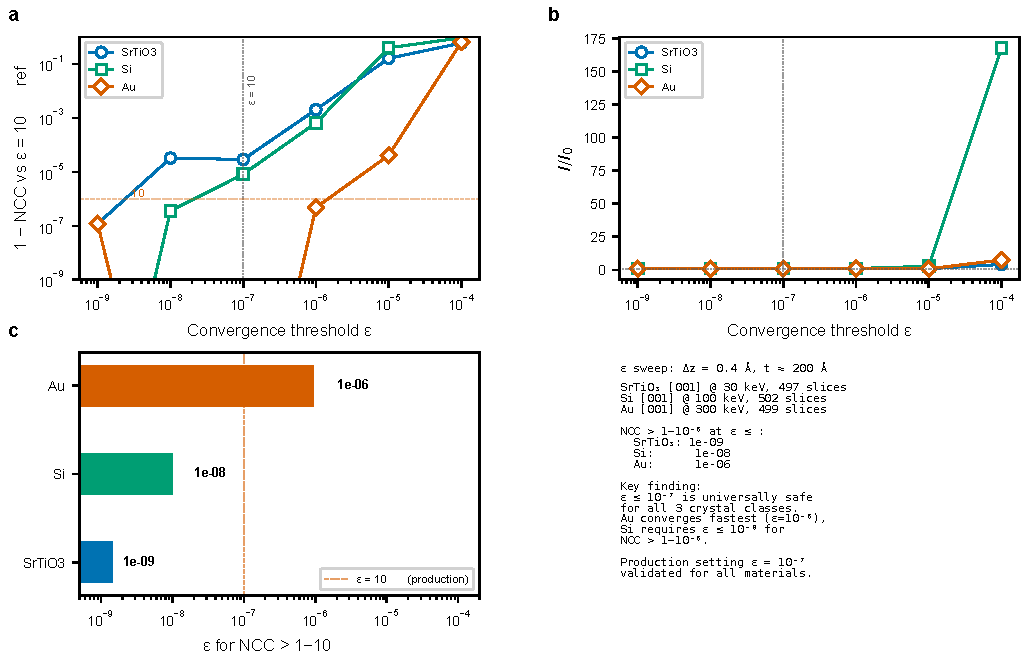
\includegraphics[width=\textwidth]{figures/c3_epsilon.pdf}
\caption{\textbf{跨材料收敛阈值敏感性。}三种材料在$\Delta z=\SI{0.4}{\angstrom}$、$t\approx\SI{200}{\angstrom}$条件下，扫描$\varepsilon\in[10^{-9},10^{-4}]$。(a) $1-$NCC随$\varepsilon$变化：Z排序的收敛速度（Au最快，Si最慢）。(b) $I/I_0$随$\varepsilon$变化：$\varepsilon=10^{-4}$时灾难性欠收敛。(c) 每种材料达到NCC $>1-10^{-6}$所需$\varepsilon$阈值。(d) 摘要：$\varepsilon\le10^{-7}$对所有三种晶体类型普遍安全。}\label{fig:epsilon_sweep}
\end{figure}

\subsection{带宽继承、抗混叠与float32精度底噪}\label{sec:bandwidth-cost}

\subsubsection{带宽继承与抗混叠}

乘积$V\psi$使$\hat\psi$的支撑集加倍，因为$\widehat{V\psi}=\hat V*\hat\psi$，而Lobato形状因子~\cite{LobatoVanDyck2014}的$q^{-2}$渐近行为确保$\hat V$具有延伸到网格Nyquist频率的厚重尾部。无带限时，K级数功率谱在$n=3$次迭代内饱和Nyquist边界。应用$\tfrac23$-Nyquist余弦锥形孔径对所有测试材料实现了带宽控制，消除了先前被误归因于Taylor级数发散的现象。

在细采样（\SI{0.05}{\angstrom\per\pixel}）下，抗混叠是强制性的：禁用抗混叠时，模拟立即溢出（所有指标为NaN/Inf）。启用抗混叠时，NCC = 0.987相对于更细$\Delta z=\SI{0.2}{\angstrom}$参考，高频功率比为$\sim10^{-15}$——确认了完全的带宽控制（补充表S5）。剩余的NCC间隙$\sim$0.013反映了$\Delta z$加倍产生的真实对易子误差，与第\ref{sec:convergence}节建立的$\mathcal O(\Delta z^2)$标度一致。


\subsubsection{Float32精度底噪}\label{sec:float32}

K级数和中的float32累积导致数值扩散：$I/I_0<1$在所有情况下成立。为映射$(\Delta z, t)$参数空间，对SrTiO$_3$ [001]在\SI{30}{\keV}下扫描了6个$\Delta z$值$\times$5个厚度（共30个点）。float32误差是扩散性的，而非放大性的——全部30次运行均显示$I/I_0<1$——每片扩散系数$\varepsilon_\text{f32}\equiv1-I/I_0^{1/n_\text{slices}}$将所有数据坍缩到相对于$n_\text{slices}$的单一曲线上，与$\Delta z$无关。线性拟合$I/I_0\approx1-\alpha\,n_\text{slices}$给出$\alpha\approx2.7\times10^{-5}$每片。

float32扩散误差和对易子误差具有相反的$\Delta z$依赖性，对可用切片厚度形成双侧约束。对易子误差按$\propto\Delta z^2$标度，更大的$\Delta z$产生更大误差，设定上界。float32扩散按$\propto n_\text{slices}=t/\Delta z$标度，更细的$\Delta z$意味着更多切片、更多累积，设定下界。对于$I/I_0>0.99$，float32约束要求$n_\text{slices}<330$，即在$t=\SI{200}{\angstrom}$时$\Delta z\ge\SI{0.6}{\angstrom}$。结合对易子约束NCC $>0.99$要求$\Delta z\le\SI{0.7}{\angstrom}$（来自第\ref{sec:channeling-holz}和\ref{sec:operating-envelope}节），SrTiO$_3$在\SI{30}{\keV}下的最优$\Delta z$窗口为0.6--0.7~\AA{}——比传统的0.4--1.0~\AA{}范围更窄，且现在有了定量依据（图\ref{fig:float32}）。

\begin{figure}[H]
\centering
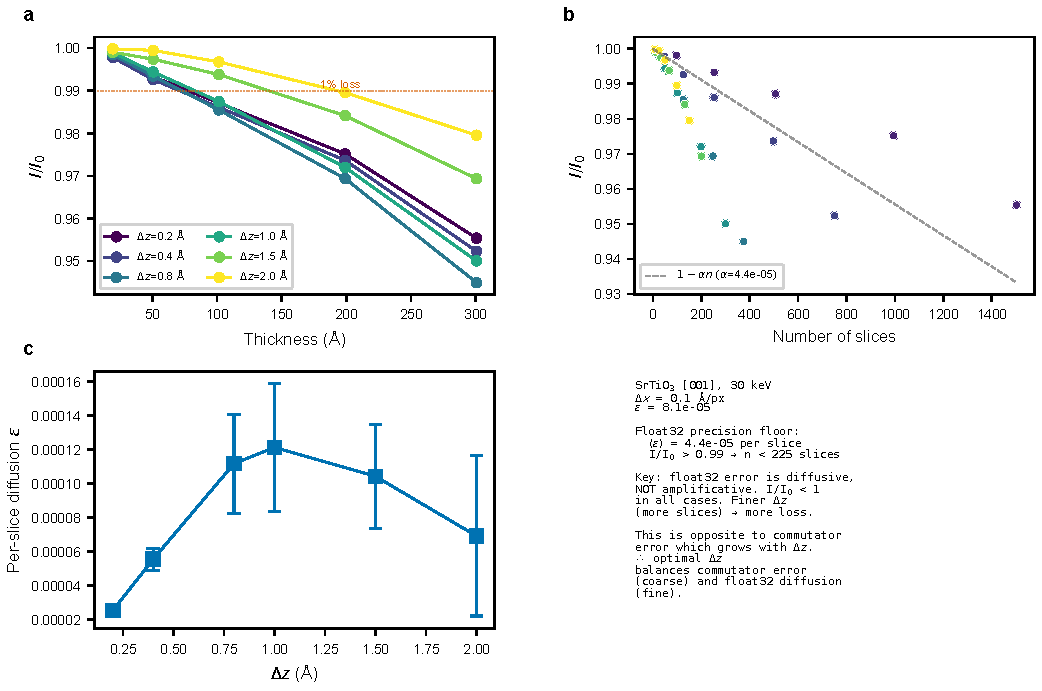
\includegraphics[width=\textwidth]{figures/c8_float32.pdf}
\caption{\textbf{Float32精度底噪。}(a) 各$\Delta z$下$I/I_0$随厚度变化。(b) 相对于$n_\text{slices}$的数据坍缩。(c) 每片扩散$\varepsilon_\text{f32}$随$\Delta z$变化。(d) 总结：平衡对易子误差（上界）和float32扩散（下界）的双侧最优$\Delta z$窗口。}\label{fig:float32}
\end{figure}


% ═══════════════════════════════════════════════════════════
\section{讨论}
% ═══════════════════════════════════════════════════════════

发散比$r(\mathbf{R})=\sum|w|/\sum|\psi_\text{exit}|$在数学上是下一个Taylor项的控制器。物理上，第\ref{sec:diagnostic-potential}节的二维图揭示$r$是$V(\mathbf{R})$和$\nabla_\perp V(\mathbf{R})$的\textbf{局域探针}：$r$峰值像素与原子柱位置重合，峰高在Sr、Ti、O和间隙位置上追踪$\sigma V_\text{col}\Delta z$。K级数恰好在局域散射项$\sigma V\psi$在单片内压倒衍射平滑$\nabla_\perp^2\psi/(4\pi K_0)$时失败——即当切片厚度超过局域平均自由程$\ell_\text{mfp}=1/(\sigma V_\text{rms})$时。用第\ref{sec:length-scales}节的长度尺度语言来说，当$\rho=\Delta z/\ell_\text{mfp}\gtrsim1$时出现发散，而当额外满足$\eta=r_F/w_\text{col}<1$时，停滞作为前兆信号出现。

这一行为的物理根源在于传统分裂方法丢弃的对易子。Lie--Trotter分裂$\exp(i\Delta z\hat A)\exp(i\Delta z\hat B)$以每片$-\tfrac12\Delta z^2[\hat A,\hat B]+\mathcal O(\Delta z^3)$的代价替代$\exp(i\Delta z(\hat A+\hat B))$，全局累积为$\mathcal O(\Delta z)$。这可从Baker--Campbell--Hausdorff（BCH）公式直接看出
\begin{equation}\label{eq:bch}
\exp(A)\exp(B)=\exp\!\big(A+B+\tfrac12[A,B]+\tfrac{1}{12}[A,[A,B]]-\tfrac{1}{12}[B,[A,B]]+\cdots\big),
\end{equation}
该公式将对易子$[\hat A,\hat B]$确定为指数中$A+B$之外的主导阶项。Strang~\cite{Strang1968}证明对称分裂通过消除这一主导对易子项将每步误差降至$\mathcal O(\Delta z^3)$，但正如McLachlan和Quispel~\cite{McLachlanQuispel2002}所述，当对易子不可忽略时，没有一种分裂方案能同时达到高精度和高效率，因为高阶BCH项不能同时全部消除。B\'atkai\textit{等}~\cite{Batkai2009}通过Trotter--Kato定理提供了收敛分析，证实分裂误差由$\|[\hat A,\hat B]\|$控制。

取$\hat A=\sigma V$和$\hat B=\nabla_\perp^2/(4\pi K_0)$，对易子
\begin{equation}\label{eq:commutator}
[\hat A,\hat B]\propto\nabla_\perp V\!\cdot\!\nabla_\perp+\tfrac12\nabla_\perp^2 V
\end{equation}
尖锐地局域在原子柱上——恰是通道效应局域化和HOLZ Bloch态耦合发生之处~\cite{ChenVanDyck1997,PennycookNellist2011}。第\ref{sec:channeling-holz}节的$\Delta z$扫描揭示，CVDMS与Fourier多层法之间的Pendell\"osung周期差异出现在$\Delta z=\SI{0.8}{\angstrom}$（$\Delta\xi=\SI{3.2}{\angstrom}$）并在$\Delta z=\SI{1.0}{\angstrom}$（$\Delta\xi=\SI{2.0}{\angstrom}$）持续存在，而在$\Delta z\le\SI{0.4}{\angstrom}$处两种方法不可区分。这种随$\Delta z$变化的分歧是被忽略对易子的\textbf{直接实验特征}——不是一般的数值误差。CVDMS通过Taylor级数将$[\hat A,\hat B]$保留到$\Delta z$的所有阶，在粗切片下放大对易子信号，并提供逐像素诊断量（$r(\mathbf{R})$、$s(\mathbf{R})$），预测分裂近似\textit{在何处和何时}将失效，早于其传播到可观测量之前。

转向与现有方法的关系，传统Fourier多层法~\cite{Kirkland2020,CowleyMoodie1957,MadsenSusi2021}精确守恒$\|\psi\|$，并在abTEM~\cite{MadsenSusi2021}、PRISM~\cite{Ophus2017}和MULTEM~\cite{LobatoVanDyck2015}中得到了充分验证；其对易子误差通过减小$\Delta z$直到结果停止变化来控制——这是一种\textbf{间接的}、全局的收敛测试，需要多次运行且无法定位误差来源。Bloch波方法~\cite{Kirkland2020}通过保留的束数控制精度，为轴向通道效应提供了自然的参考，但要求周期性势且在HRTEM尺度的束数下计算代价高昂。CVDMS可追溯到Coene和Van Dyck~\cite{CoeneVanDyck1984}的实空间多层法算法，该算法在二维网格上使用有限差分Laplacian。Wacker和Schr\"oder~\cite{WackerSchroder2015}系统比较了实空间和Fourier空间多层法算法，讨论了Laplacian离散化精度——这一问题被本工作的FD/FFT双后端设计直接继承（第\ref{sec:laplacian}节）。CVDMS通过为同一算符$\hat{K}$提供FD和FFT两种Laplacian后端，桥接了这两个传统。因此它在现有方法中占据第三位置：保留了多层法的几何灵活性，同时\textbf{原位暴露}了原本隐藏的对易子误差作为逐像素量，使收敛性成为样品在每个点上的属性，而非整个模拟的属性。我们将其作为一种\textbf{不同的受控近似}，而非分裂方法或Bloch波方法的替代品。

对于普通TEM从业者，本研究的可操作输出有三个方面。第一，生产默认值$\Delta z=\SI{0.4}{\angstrom}$、$\varepsilon=10^{-7}$现在得到了定量验证而非启发式采纳：它在全部三类晶体中提供NCC $>1-10^{-5}$，且安全地位于双侧最优窗口分析所识别的对易子-发散阈值下方（对SrTiO$_3$在\SI{30}{\keV}下为0.6--0.7~\AA{}，第\ref{sec:float32}节）。第二，逐像素诊断量使得\textbf{单次$\Delta z$选择}成为可能：用户可运行一次模拟并检查$n^*(\mathbf{R})$和$r(\mathbf{R})$来识别需要局域$\Delta z$细化的区域，取代传统的多次$\Delta z$扫描收敛测试。第三，$t=\SI{200}{\angstrom}$处的Z主导收敛（第\ref{sec:operating-envelope}节）提供了简单的材料依赖指南：轻元素（$Z\lesssim14$）在标准参数下无条件收敛；中等元素（$Z\sim38$）需要监测停滞诊断量；重元素（$Z\gtrsim79$）无论其他参数如何选择都需要减小$\Delta z$或使用float64精度。在此之外，$(\rho,\eta)$参数化（第\ref{sec:operating-envelope}节）提供了量纲正确的收敛阈值，而非全局$\Delta z$经验规则：同一网格上的SrTiO$_3$薄膜和Au团簇接受不同的有效$\Delta z$容限，区域边界由仅从结构因子$V_g$可估算的长度比设定。$V(\mathbf{R})\leftrightarrow n^*(\mathbf{R})$关联（第\ref{sec:diagnostic-potential}节）为自适应切片开辟了道路，仅在诊断量标记处细化$\Delta z$而非全局细化——通过单次CVDMS运行即可实现，该运行同时产生出射波和$n^*(\mathbf{R})$图，标识哪些像素需要更细切片。Fresnel BSC残差为异质结构界面建模提供了可直接测量的量，扩展到真空/样品和衬底/样品边界，简化背散射近似在这些界面可产生$\sim$17\%的通量误差，传播到下游CBED盘中。对于目前使用Bloch波参考~\cite{Kirkland2020,PennycookNellist2011,Allen2003}的定量衍射分析，第\ref{sec:channeling-holz}节的通道效应和HOLZ可观测量确立了CVDMS与Fourier多层法在标准生产$\Delta z\le\SI{0.4}{\angstrom}$下不可区分，而可测量的对易子驱动分歧仅在$\Delta z\ge\SI{0.8}{\angstrom}$出现——表明常规切片厚度下的常规多层法已经捕获了相关的通道效应物理，逐像素诊断量提供了一个\textit{先验}指标，指示何时需要更细切片。最后，对于重元素低电压场景（如Au在\SI{30}{\keV}下），float32抵消构成任何算法的精度底噪——而非CVDMS的局限——建议使用float64 K级数作为补救措施。

几项局限性界定了本研究当前的范围。非弹性过程（等离激元、声子~\cite{Forbes2010}）需要单独处理；CVDMS提供了弹性基础，下文讨论的IPR诊断量是与声子通道耦合的自然起点。投影势前提依然存在：诊断量指示投影近似何时失效，但不修复它；在发散区域（$\rho\gg1$），需要全三维方法~\cite{LobatoVanDyck2014}。在同等收敛设置下，每片代价超过Lie--Trotter多层法——这是内K级数和逐像素诊断量的代价；因此CVDMS的产出不是在固定$\Delta z$下更快的墙上时间，而是能够\textbf{认证}样品上的局域收敛性，并在模拟完成前识别Lie--Trotter结果将默默继承被忽略对易子的区域。定量论断基于三类晶体（轻共价键Si、混合离子SrTiO$_3$、重金属Au）和三种能量（30/100/300~keV）；外推到二维材料、非晶样品或低于\SI{30}{\keV}的束流需要重新运行Phase~0.5协议，诊断量本身不保证验证包络外的精度。未来工作包括由实时$n^*(\mathbf{R})$驱动的自适应$\Delta z$、混合精度K级数、与声子和叠层衍射4D-STEM工作流~\cite{Savitzky2021}的耦合，以及扩展到背散射主导的RHEED。

三个守恒可观测量为CVDMS框架提供了独立的交叉检验。\label{sec:conserved-observables}逆参与比$\text{IPR}(z)=\sum|\psi|^4/(\sum|\psi|^2)^2$追踪原子柱上束流局域化的程度；对SrTiO$_3$在\SI{30}{\keV}下，有BSC的CVDMS平均IPR$\times$面积$=11.2$，无BSC的CVDMS亦为$11.2$，确认背散射在此能量下不扰动通道效应态。逐像素连续性残差$|\partial_z|\psi|^2+\nabla_\perp\cdot\mathbf{j}_\perp|$与局域势$V(\mathbf{R})$相关（$V$与逐像素最大残差之间的Pearson $r=0.74$，补充数据~P6），与对易子误差在势梯度最陡处最大的解释一致。对于实验可获取的$\{200\}$、$\{220\}$、$\{420\}$ CBED盘强度（在对称孔径上积分，补充数据~P5）：在$t\le\SI{200}{\angstrom}$时，CVDMS相对于$\Delta z\to0$ Fourier参考的偏差在所有三个盘中$<6\%$；$\{200\}$盘——最强且最具实验相关性——在$t\le\SI{400}{\angstrom}$时偏差$<4\%$；高阶盘$\{220\}$和$\{420\}$在更大厚度处显示递增的对易子敏感性（在$t\approx\SI{390}{\angstrom}$时分别为16\%和36\%），与其更大的散射矢量采样更细空间频率一致，而投影势近似在这些频率处退化。

% ═══════════════════════════════════════════════════════════
\section{方法}
% ═══════════════════════════════════════════════════════════

\subsection{控制方程与算符$\hat{K}$}

快电子的相对论修正标量波方程可写为~\cite{ChenVanDyck1997}
\begin{equation}\label{eq:KE}
\hat{K}(\mathbf{r})=K_0\sqrt{1+\frac{\nabla_\perp^2}{(2\pi K_0)^2}+\frac{\sigma\,U(\mathbf{r})}{\pi K_0}},
\end{equation}
其中$K_0=1/\lambda$为相对论波数，$\sigma=2\pi m e\lambda/h^2$为相互作用常数。在切片$j$内，投影势$V_j(\mathbf{R})=\int_{(j-1)\Delta z}^{j\Delta z}U(\mathbf{r})\,dz$定义切片散射算符
\begin{equation}\label{eq:Kj}
\hat{K}_j\psi(\mathbf{R})=\sigma\,V_j(\mathbf{R})\,\psi(\mathbf{R})+\frac{\nabla_\perp^2\psi(\mathbf{R})}{4\pi K_0}.
\end{equation}

\subsection{切片传播子的双重Taylor展开}

前向传播子通过直接指数化计算：
\begin{equation}\label{eq:taylor}
\psi_{j+1}=\exp\!\big(i\,\Delta z\,\hat{K}_j\big)\,\psi_j
=\sum_{n=0}^{\infty}\frac{(i\,\Delta z)^n}{n!}\,\hat{K}_j^{\,n}\psi_j.
\end{equation}
内部幂次$\hat{K}_j^{\,n}\psi$通过二项式平方根级联计算，系数为
\begin{equation}\label{eq:cn}
c_1=1,\qquad c_n=\frac{(0.5-n+1)\,\lambda}{\pi\,n},\quad n>1.
\end{equation}
利用$\hat{K}$的线性性——$\hat{K}(c\psi)=c\,\hat{K}(\psi)$——该级联以\textbf{标度形式}实现
\begin{equation}\label{eq:cascade}
\mathrm{cur}_n=c_n\,\hat{K}_j(\mathrm{cur}_{n-1}),\qquad
\hat{K}_j^{\,n}\psi\approx\sum_{m=1}^{n}\mathrm{cur}_m,
\end{equation}
将系数阻尼传播到每个高阶项，并防止在典型TEM参数下float32算术中$\hat{K}_j^{\,n}\psi$的虚假溢出。

\subsection{逐像素收敛诊断量}

三个逐像素场与出射波一并报告：

\textbf{外发散比}$r(\mathbf{R})$（默认截断值5.0）：
\begin{equation}\label{eq:divergence-ratio}
r=\frac{\sum|w|}{\sum|\psi_{\text{exit, before}}|},
\end{equation}
其中$w=(i\Delta z)^n\hat{K}^{\,n}\psi/n!$为候选的第$n$个外Taylor项，分母在添加新项之前计算以避免人为约束在1附近。逐像素地，使$r$降至逐像素容差$\varepsilon$以下的最小$n$定义为$n^*(\mathbf{R})$。

\textbf{内K级数停滞计数。}在一个外项内，内级联持续迭代直到超阈值像素数$n_\text{above}$在连续K迭代之间停止减少；逐像素停滞计数$s(\mathbf{R})$以停滞图形式报告。

\textbf{Fresnel BSC幺正残差。}在每个切片边界计算图$\mathcal{U}(\mathbf{R})=|T(\mathbf{R})|^2+|R(\mathbf{R})|^2-1$（第\ref{sec:bsc}节）。

\subsection{带限}\label{sec:bandlimiting}

乘积$V\psi$通过$\widehat{V\psi}=\hat V*\hat\psi$使带宽加倍——这是一种可在标量衍射理论的角谱框架内理解的带宽继承效应~\cite{Goodman2017}。Lobato形状因子~\cite{LobatoVanDyck2014}的$q^{-2}$渐近行为确保$\hat V$具有延伸到网格Nyquist频率的厚重尾部，使抗混叠成为物理必需而非装饰性滤波。追溯至Self\textit{等}~\cite{Self1983}建立的带限实践，$\tfrac23$-Nyquist余弦锥形孔径在K展开前对投影势施加一次，并在每次$\hat{K}$应用后施加（默认）。FD和FFT Laplacian路径共享同一孔径。

\subsection{Laplacian后端}\label{sec:laplacian}

CVDMS实现提供了四种精度递增的有限差分Laplacian和一个FFT Laplacian。FD精度8（9点可分离1D模板）为默认值，提供精度与计算效率之间的最优平衡。


\subsection{通量守恒Fresnel背散射修正}\label{sec:bsc}

在切片$j$和$j+1$之间的界面处，$\psi$和$\partial_z\psi$跨越$\hat{K}_j$不连续点的连续性给出
\begin{equation}\label{eq:fresnel-bsc}
R=\frac{\hat{K}_j-\hat{K}_{j+1}}{\hat{K}_j+\hat{K}_{j+1}},\qquad
T=\frac{2\,\hat{K}_j}{\hat{K}_j+\hat{K}_{j+1}},\qquad
|T|^2+|R|^2=1,
\end{equation}
我们在$\Delta z\,\nabla V$的一阶下数值计算上述公式。传统的简化背散射近似$T=1-B$在$B<0$时违反幺正性，此处仅作为有文档记录的负对照。

\subsection{数值实现}

\textbf{公共API：}{\tt CVDMSMultislice(...)}通过abTEM~\cite{MadsenSusi2021}中的{\tt probe.multislice(potential, algorithm=cvdms)}访问。

\textbf{后端选择：}{\tt backend="auto"}在可用时尝试C++/CUDA；否则回退到CuPy/Python路径。

\textbf{C++/CUDA实现：}将Laplacian + $\hat{K}$ + 标度级联存储 + 累积 + 收敛计数融合为单个核函数。BSC调度使用两个CUDA流，为$V_\text{cur}$和$V_\text{next}$重叠K级数工作。

\textbf{默认参数：}外Taylor最大30，内K级数最大30，$\varepsilon=10^{-7}$，发散比5.0，停滞耐心2，FD精度8，AA孔径$\tfrac23$ Nyquist，complex64。

\subsection{测试系统与参考模拟}\label{sec:test-systems}

\textbf{晶体系统。}SrTiO$_3$ [001]（默认基准，$a=\SI{3.905}{\angstrom}$，627$\times$627网格，\SI{0.044}{\angstrom\per\pixel}），Si [001]（$a=\SI{5.431}{\angstrom}$，627$\times$627网格，$\approx\SI{0.039}{\angstrom\per\pixel}$），Au [001]（$a=\SI{4.078}{\angstrom}$，627$\times$627网格，$\approx\SI{0.033}{\angstrom\per\pixel}$）；均为$4\times4\times N$超胞，每个原子柱$\ge6$个像素。对于参数扫描（C系列），使用\SI{0.10}{\angstrom\per\pixel}采样，以在可控计算代价下对所有材料进行系统性的$(\Delta z, t, \varepsilon)$变化。

\textbf{默认切片厚度。}$\Delta z=\SI{0.4}{\angstrom}$（在$t=\SI{100}{\angstrom}$时$N_z=250$，在$t=\SI{400}{\angstrom}$时$N_z=1000$）。

\textbf{参考方法。}abTEM Fourier多层法~\cite{MadsenSusi2021}，采用$\Delta z\to0$外推（complex128），匹配带限和投影势参数化（Lobato参数化~\cite{LobatoVanDyck2014}）。

\subsection{统计与不确定性报告}

精度指标：归一化互相关（NCC）被选为主要波函数级指标，因为它同时对振幅和相位差异敏感——不同于仅探测总强度的$I/I_0$——且是电子显微学出射波重建中的标准比较器。NCC对全局相位偏移和均匀振幅标度不敏感；相位RMS和$I/I_0$与NCC一并报告以捕捉这些误差模式。衍射图案NCC在线性强度CBED图案上计算，不进行阈值化或对数标度。

本文报告的所有C系列和P系列参数扫描均使用单构型Debye--Waller展宽静态势$V^{(B)}$；此处引用的冻结声子系综大小$N\ge8$是指推荐用于实验数据比较的统计协议，而非第\ref{sec:convergence}--\ref{sec:bandwidth-cost}节的收敛验证数据。收敛统计量：$n_\text{above}$、$n_\text{nan}$、$n_\text{diverging}$每片记录，并以中位数和95\%区间跨探针扫描进行汇总。三种材料在匹配参数设置下的系统性墙上时间基准测试将在专注于GPU性能优化的后续工程论文中报告。

\subsection{投影势场：参数化、热展宽与柱结构}\label{sec:potential-field}

切片势按原子构建为$V_j(\mathbf{R})=\sum_a V_a(\mathbf{R}-\mathbf{R}_a^{\perp})\,\Pi_j(z_a)$，其中$V_a$为投影单原子静电势，$\Pi_j$为切片隶属窗口。全文使用Lobato和Van Dyck参数化~\cite{LobatoVanDyck2014}；在可用参数化中，它提供了对相对论Hartree--Fock散射因子在完整$q$范围内最精确的解析拟合，正确再现了大$q$处的$q^{-2}$渐近衰减——这一性质对第\ref{sec:bandlimiting}节的带限分析至关重要。

两个物理场进入分析：(i) \textbf{静态势}$V^{(0)}(\mathbf{R})$——用于包络和长度尺度测量；(ii) \textbf{热展宽势}$V^{(B)}(\mathbf{R})$——通过在倒空间施加Debye--Waller因子$\exp(-Bq^2/4)$获得。由此导出以下柱局域场：$|\nabla_\perp V|$、$\nabla_\perp^2 V$、柱宽度$w_\text{col}$（FWHM）、柱峰值$V_\text{col}$和间隙均值$V_\text{gap}$。

% ═══════════════════════════════════════════════════════════
\section*{数据可用性}
局部模拟输出写入{\tt docs/data/}（HDF5/NPZ；通过{\tt .gitignore}排除在版本控制之外）。本研究中使用的所有出射波数组、CBED图案、收敛诊断日志和基准测试时间数据将存放在\textit{Zenodo}上，DOI可供匿名审稿人访问。

% ═══════════════════════════════════════════════════════════
\section*{代码可用性}
CVDMS实现存档于\textit{Zenodo}，DOI [待分配]。活跃开发版本托管于{\tt https://github.com/<org>/abTEM-cvdms}，使用GPL-3.0许可证。每幅图和每个表使用的精确提交标记为{\tt cvdms-comms-phys-v1}。

% ═══════════════════════════════════════════════════════════
\section*{致谢}
[待补充：资金来源、项目编号、计算资源分配。]

% ═══════════════════════════════════════════════════════════
\section*{作者贡献}
\textbf{CRediT分类法：}概念构思---G.S.C.和Y.T.H.；方法学---G.S.C.；软件---G.S.C.；验证---J.Y.和G.S.C.；形式分析---J.Y.和G.S.C.；调查---J.Y.和G.S.C.；资源---Y.T.H.；写作（初稿）---G.S.C.；写作（审阅与编辑）---J.Y.、Y.T.H.和G.S.C.；可视化---J.Y.和G.S.C.；指导---Y.T.H.；资金获取---Y.T.H.

% ═══════════════════════════════════════════════════════════
\section*{利益冲突}
作者声明无利益冲突。

% ═══════════════════════════════════════════════════════════
\bibliographystyle{unsrtnat}
\bibliography{cvdms_references}

\end{document}
